\documentclass[11pt]{article}
% This file will be kept up-to-date at the following GitHub
%  repository: https://github.com/alexhernandezgarcia/latex-simple
%  Please file any issues/bug reports, etc. you may have at:
%  https://github.com/alexhernandezgarcia/latex-simple/issues

\usepackage{microtype} % microtypography
\usepackage{booktabs} % tables
\usepackage{url} % urls

% AMS math
\usepackage{amsmath} \usepackage{amsthm} \usepackage{amssymb}

% With no package options, the submission will be anonymized, the
%  supplemental material will be suppressed, and line numbers will be
%  added to the manuscript.  To hide the supplementary material (e.g.,
%  for the first submission deadline), use the [hidesupplement]
%  option: \usepackage[hidesupplement]{latex-simple} To compile a
%  non-anonymized camera-ready version, add the [final] option (for
%  the main track) e.g., \usepackage[final]{latex-simple} or
%  \usepackage[final, hidesupplement]{latex-simple}

\usepackage[final]{latex-simple}

% You may use any reference style as long as you are consistent
%  throughout the document. As a default we suggest author--year
%  citations; for bibtex and natbib you may use:

\usepackage{natbib}

% and for biber and biblatex you may use:

% \usepackage[% backend=biber, style=authoryear-comp, sortcites=true, natbib=true, giveninits=true, maxcitenames=2, doi=false, url=true, isbn=false, dashed=false ]{biblatex} \addbibresource{...}

\usepackage{chessboard} \usepackage{skak} \usepackage{float}
\usepackage{tikz}
\ExplSyntaxOn %requires texlive 2020, in older system load expl3
\cs_new:Npn \getfieldnumber #1 { \fp_eval:n { (\tl_tail:V #1 -1)*8 +
    \exp_args:Ne\int_from_alph:n{\tl_head:V #1} -1} } \ExplSyntaxOff

\title{GFlowChess: Joueur d'échec basé sur GFlowNet et sur Stockfish}

% The syntax for adding an author is \author[i]{\nameemail{author
%  name}{author email}} where i is an affiliation counter. Authors may
%  have multiple affiliations; e.g.:
%  \author[1,2]{\nameemail{Anonymous}{anonymous@example.com}}
\author[1]{\nameemail{Yizhan Li}{yizhan.li@umontreal.ca}}
\author[1]{\nameemail{Olivier
    Déry-Prévost}{olivier.dery-prevost@umontreal.ca}}
\author[1]{\nameemail{Sidya Galakho}{sidya.galakho@umontreal.ca}}
\author[1]{\nameemail{Simon Théorêt}{simon.theoret.1@umontreal.ca}}

% the list might continue: \author[2,3]{\nameemail{Author
%  2}{email2@example.com}} \author[3]{\nameemail{Author
%  3}{email3@example.com}} \author[4]{\nameemail{Author
%  4}{email4@example.com}}

% if you need to force a linebreak in the author list, prepend an
%  \author entry with \\:

% \author[3]{\\\nameemail{Author 5}{email5@example.com}}

% Specify corresponding affiliations after authors, referring to
%  counter used in \author:

\affil[1]{Université de Montréal}

% the list might continue: \affil[2]{Institution 2}
%  \affil[3]{Institution 3} \affil[4]{Institution 4}

% define PDF metadata, please fill in to aid in accessibility of the
%  resulting PDF
\hypersetup{%
  pdfauthor={}, % will be reset to "Anonymous" unless the "final" package option is given
  pdftitle={}, pdfsubject={}, pdfkeywords={} }

\begin{document}

\maketitle

% CCC: Contexte Contenu Conclusion

\begin{abstract}
	Dans ce rapport, nous présentons GFlowChess, un modèle basé sur la
	famille de modèle GFlownet capable de simuler une partie d'échec
	suivant les règles traditionnelle du jeu. Nous évaluons la
	performance du modèle à l'aide de Stockfish, un moteur d'échec
	moderne capable d'évaluer la probabilité de victoire d'un
	match. Nous avons testé 2 types de pertes ainsi que deux fonctions
	de récompenses pour observer le déroulement des trajectoires. Nous
	avons en effet été en mesure de constater les effets des fonctions
	de récompenses sur la distribution des trajectoires échantillonnées
	et de favoriser un joueur ou bien un autre.
\end{abstract}

\subsection{GFlowNet}
Les réseaux de flux génératifs (GFlowNets) sont des modèles
d'échantillonnage séquentiels formés pour correspondre à une
distribution donnée, où les flux peuvent représenter chaque étape dans
les transitions stochastiques de l'environnement comme des actions du
GFlowNet tirées d'une politique fixe. Intuitivement, nous imaginons
que jouer aux échecs avec des GFlowNets pourrait être un bon cas
d'utilisation et un GFlowNet peut être entraîné pour simuler la
distribution d'une fonction de récompense.

\subsection{Stockfish}
Nous obtenons la fonction de récompense des échecs de Stockfish, un
moteur d'échecs open-source, qui utilise une variété d'algorithmes
pour évaluer les positions et faire des mouvements. Il peut donner un
score de chaque étape en fonction de la qualité de l'étape dans le
plateau actuel. C'est l'un des meilleurs algorithmes de récompense
incluant des techniques comme l'élagage alpha-bêta, la recherche de
variation principale, la recherche de quiescence et diverses
heuristiques pour l'évaluation des positions.

\subsection{Perte TB}
La perte d'équilibre de trajectoire (Trajectory Balance loss) est
l'objectif qui peut définir une politique qui échantillonne exactement
de la distribution cible efficacement. Cet objectif est calculé sur
des séquences d'actions complètes échantillonnées (trajectoires) de
l'état initial à un état terminal, contrairement aux objectifs de
correspondance de flux et d'équilibre détaillé.
\\
\section{Entraîner avec succès un modèle GFlowNet}
Actuellement, nous avons développé des méthodes clés pour
l'environnement de jeu, notamment l'initialisation de l'environnement,
la définition de l'espace des actions, la génération d'un masque des
actions invalides ,l'exécution d'un pas du jeu et la génération des
parents d'un état. Nous avons également mis en place un proxy pour
l'analyse des positions avec Stockfish.

Ce document décrit nos avancées jusqu'à présent, les résultats et les
défis rencontrés. En combinant les capacités de GFlowNet et de
Stockfish, notre objectif est de créer un joueur d'échecs compétitif
capable de rivaliser avec lui-même.
\subsection*{Description et résultat des méthodes développées :}

%Actuellement, les méthodes suivantes ont été développées :

%\textbf{Initialisation de l'environnement :} \\
%L'environnement GFlowChess est initialisé en prenant en compte la
% position initiale du jeu
% sur %l'échiquier. Par défaut, une position traditionnelle est utilisée, avec la notation FEN suivante : \texttt{'rnbqkbnr/pppppppp/8/8/8/8/PPPPPPPP/RNBQKBNR w KQkq - 0 1'}

%\begin{figure}[H]
%\centering
%\setchessboard{showmover=false}
%\newgame
%\chessboard
%\caption{position initial du tableau d'échiquier}
%\end{figure}

%Dans la figure 1 nous avons la position initial du tableau
% d'échiquier correspondant à la notation
% FEN %suivante : \texttt{'rnbqkbnr/pppppppp/8/8/8/8/PPPPPPPP/RNBQKBNR w KQkq - 0 1'}.  Dans cette notation les rangées du tableau sont séparées par des "/", le nombre de case vide de droite %à gauche est représenté par des chiffres, les pièces blanches sont représentées par des lettres en %majuscules et les lettres ont les significations suivantes : \{'r': 'rook','n': 'knight','b': %'bishop','q': 'queen','k': 'king'\}

\textbf{Espace des actions :} \\
L'espace des actions est défini comme l'ensemble de toutes les actions
possibles. Une action est définie comme une paire de cases (origine,
destination) sur l'échiquier.

\begin{figure}[H]
	\centering \setchessboard{color=black,clearboard,showmover=false}
	\chessboard[ pgfstyle= {[base,at={\pgfpoint{0pt}{-0.3ex}}]text},
		text= \fontsize{1.2ex}{1.2ex}\bfseries
		\sffamily\getfieldnumber\currentwq, markboard]
	\caption{cases du tableau d'échiquier encodées en chiffres}
\end{figure}

[17,35] est un exemple d'action possible qui permet d'aller de la case
17 vers la case 35 comme illustré dans la figure 2.

\textbf{Masque des actions invalides :} \\
Un masque est généré pour indiquer les actions invalides à partir de
l'état actuel du jeu. Cela permet d'éviter de choisir des actions qui
ne respectent pas les règles du jeu.

\begin{figure}[H]
	\centering
	\begin{subfigure}[b]{0.45\textwidth}
		\centering \setchessboard{showmover=false}
		\chessboard[setfen=r5k1/1b1p1ppp/p7/1p1Q4/2p1r3/PP4Pq/BBP2b1P/R4R1K
			w - - 0 20, pgfstyle=border,markfields={d4,d6}, color=blue!50,
			colorbackfield=c5, pgfstyle=color, opacity=0.5, color=red,
			markfield={d5}]
		\caption{mouvements valides}
	\end{subfigure}
	\begin{subfigure}[b]{0.45\textwidth}
		\centering \setchessboard{showmover=false}
		\chessboard[setfen=r5k1/1b1p1ppp/p7/1p6/2p1r3/PP1Q2Pq/BBP2b1P/R4R1K
			b - - 0 20, pgfstyle=border,markfields={d4,d6}, color=blue!50,
			colorbackfield=c5, pgfstyle=color, opacity=0.5, color=red,
			markfield={d5}]
		\caption{Mouvement invalide}
	\end{subfigure}
\end{figure}

En adoptant l'encodage des cases de la figure 2, la reine Blanche à la
case 35 peut effectuer les actions : [34,33], [34,42] et [34,26] comme
montré dans la figure (a).  Donc l'action [34,18] est invalide donc il
serait masqué.

\textbf{Proxy pour l'analyse des positions :} La classe \texttt{Chess}
contient un proxy pour l'analyse des positions à l'aide du moteur
Stockfish. Présentement, nous calculons la valeur du proxy comme le
négatif de la probabilité de victoire du dernier joueur à jouer. Cette
probabilité est calculée par Stockfish.

\textbf{Résultats et défis :} \\
Nous avons été en mesure d'entraîner pour 5000 itérations un modèle
GFlowNet utilisant la perte TB. De plus, nous avons limité à 10 coups
la durée des séquences. La courbe de perte est présentée ci-dessous:
\begin{figure}[H]
	\centering 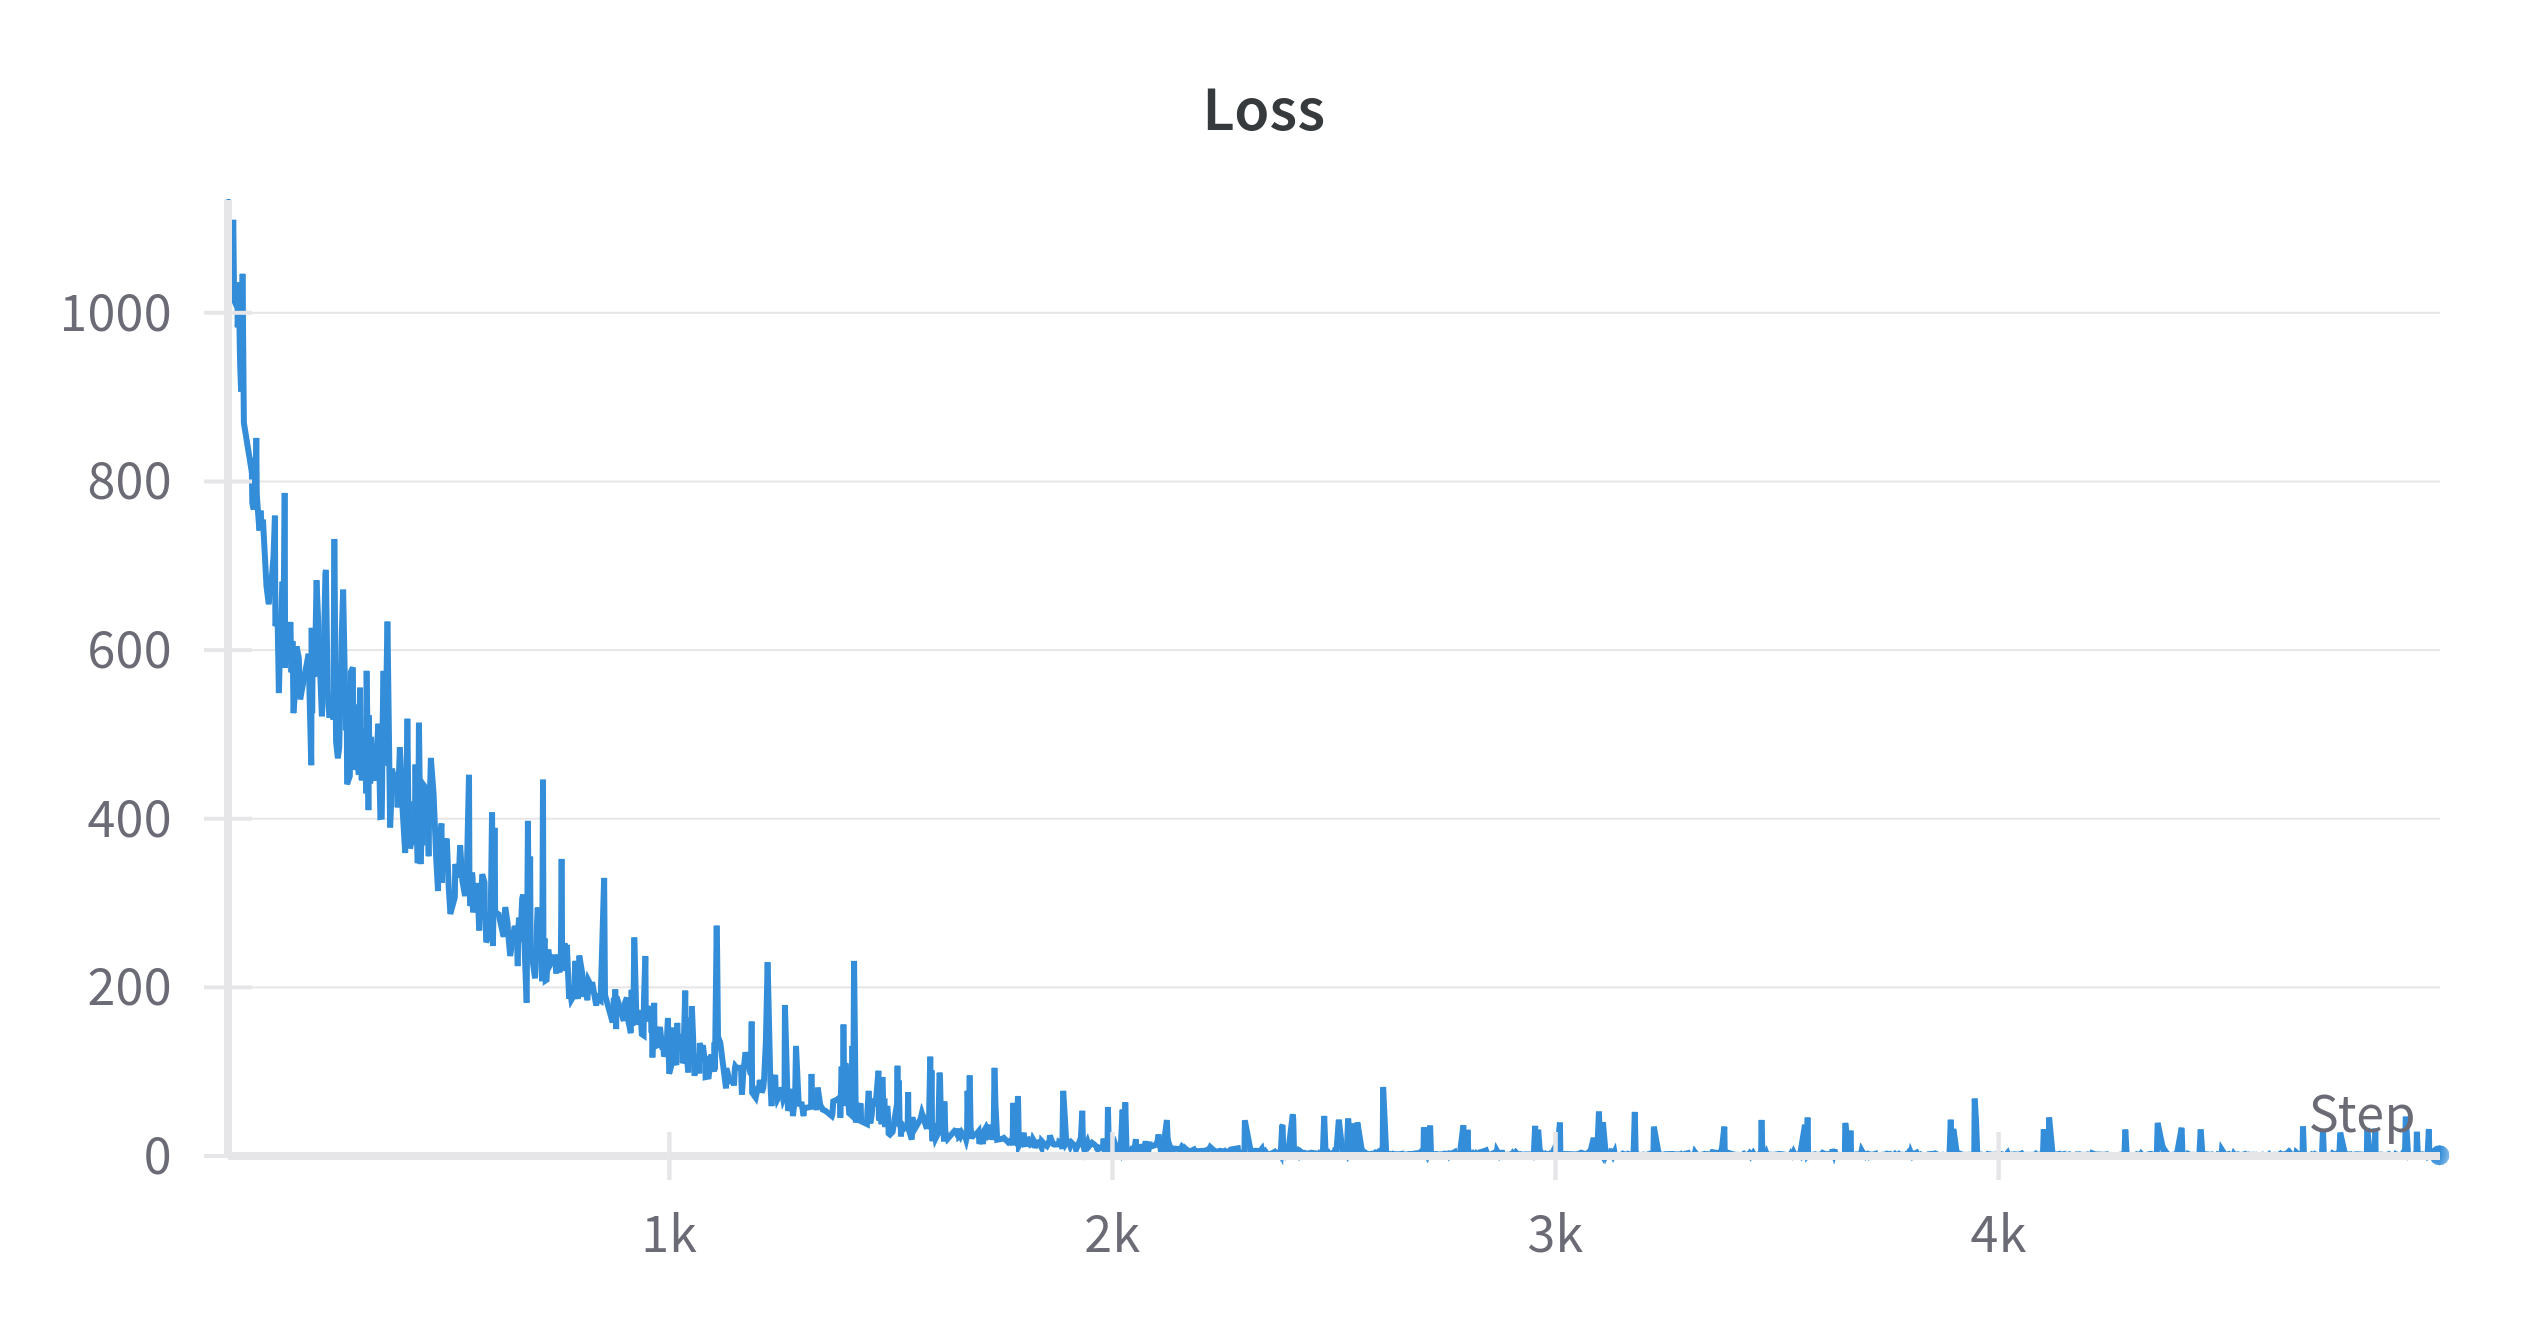
\includegraphics[scale=0.15]{tb-loss.png}
	\caption{Perte TB du modèle sur 5000 itérations}
	\label{tbloss}
\end{figure}
Or, notre modèle à encore de la difficulté à faire des ouvertures que
Stockfish juge bonne:
\begin{figure}[H]
	\centering 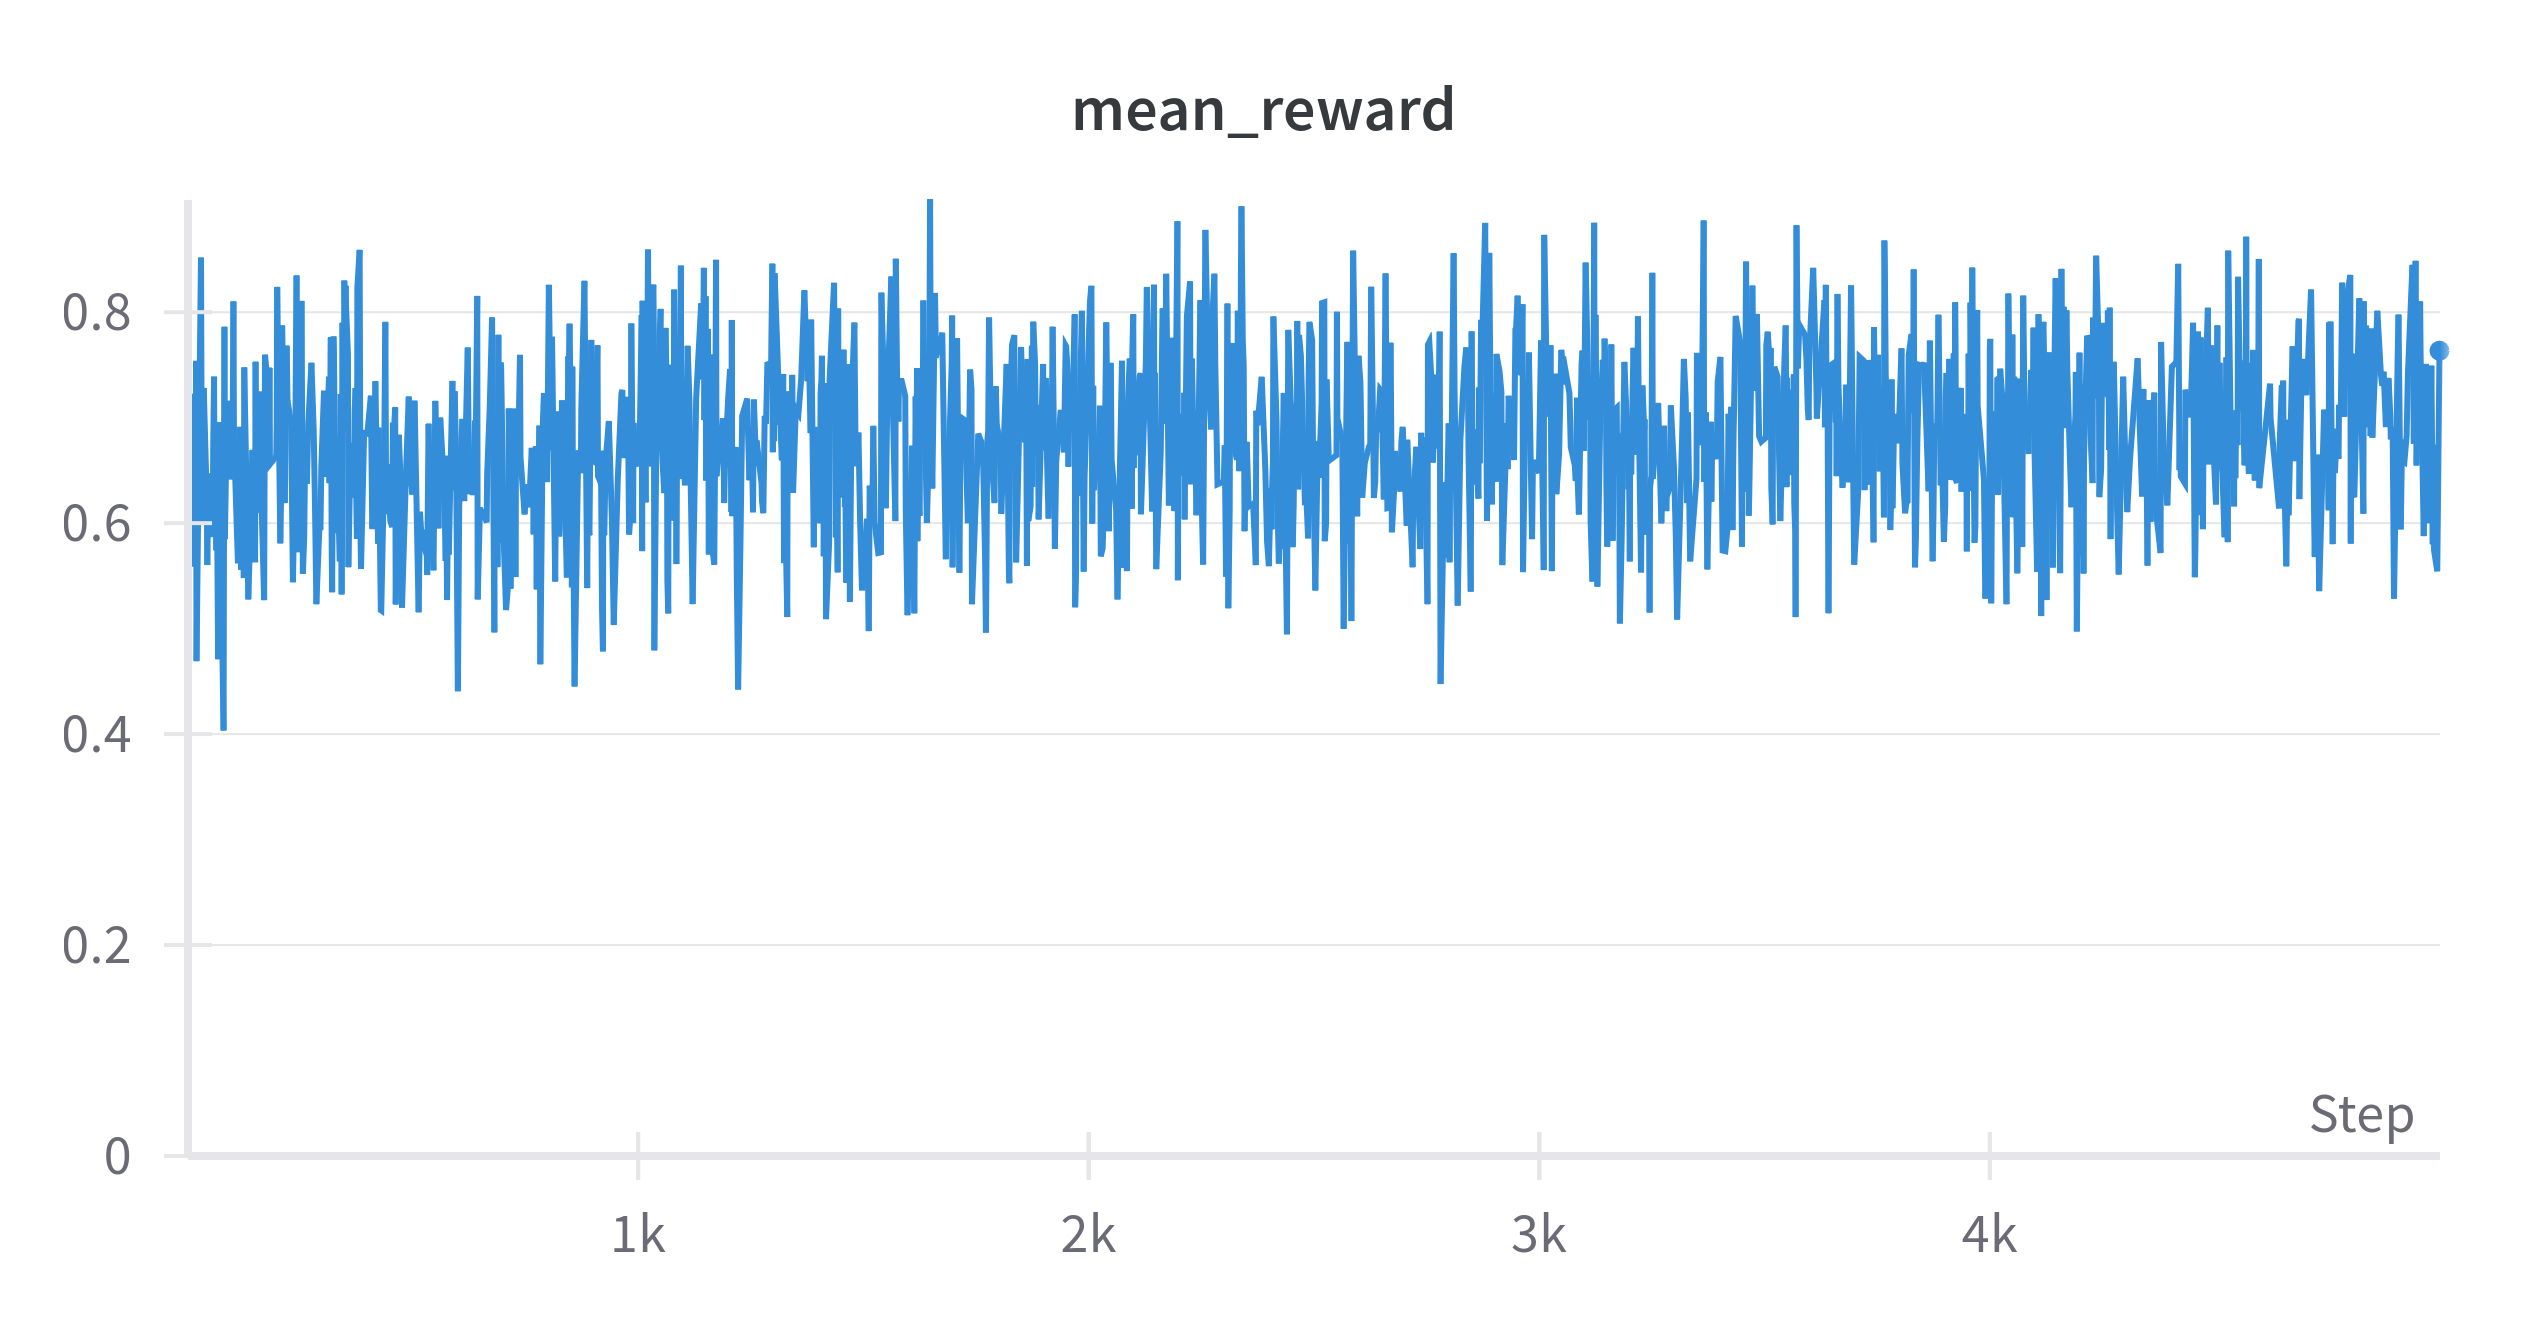
\includegraphics[scale=0.15]{tb-mean-reward.png}
	\caption{Récompense moyenne du modèle sur 5000 itérations}
	\label{tbreward}
\end{figure}
En effet, la récompense moyenne n'augmente pas durant l'apprentissage
et reste bruitée. Nous supposons que le problème est notre
\textit{proxy} actuel. En effet, notre fonction de \textit{proxy}
incite le modèle à sélectionner des coups qui avantagent le dernier
joueur à jouer (le joueur noir, dans notre cas). Au contraire, cette
fonction de \textit{proxy} incite le modèle à jouer défensivement et à
ne pas manger de pièce dès que le joueur noir à l'avantage. Une
analyse qualitative des parties échantillonnées nous pousse à croire
que cette intuition correspond à la réalité. Une fonction de
\textit{proxy} alternative consisterait à ajouter un termes positif
$\alpha d$, où $d$ représente le nombre de pièces éliminées durant une
partie et $\alpha$ correspond au poids attribué à ce terme. Ce nouveau
terme inciterait le modèle à faire des coups plus agressifs, tout en
maintenant un score Stockfish élevé.
\end{abstract}
% content will be automatically hidden during submission

% print bibliography -- for bibtex / natbib, use:


% and for biber / biblatex, use:

% \printbibliography

% supplemental material -- everything hereafter will be suppressed
%  during submission time if the hidesupplement option is provided!
\appendix

\end{document}
